\documentclass{article}


% if you need to pass options to natbib, use, e.g.:
%     \PassOptionsToPackage{numbers, compress}{natbib}
% before loading neurips_2022


% ready for submission
\usepackage[final]{neurips_2022}


% to compile a preprint version, e.g., for submission to arXiv, add add the
% [preprint] option:
%     \usepackage[preprint]{neurips_2022}


% to compile a camera-ready version, add the [final] option, e.g.:
%     \usepackage[final]{neurips_2022}


% to avoid loading the natbib package, add option nonatbib:
%    \usepackage[nonatbib]{neurips_2022}


\usepackage[utf8]{inputenc} % allow utf-8 input
\usepackage[T1]{fontenc}    % use 8-bit T1 fonts
\usepackage{hyperref}       % hyperlinks
\usepackage{url}            % simple URL typesetting
\usepackage{booktabs}       % professional-quality tables
\usepackage{amsfonts}       % blackboard math symbols
\usepackage{nicefrac}       % compact symbols for 1/2, etc.
\usepackage{microtype}      % microtypography
\usepackage{xcolor}         % colors
\usepackage{graphicx}


\title{Homework 2}


% The \author macro works with any number of authors. There are two commands
% used to separate the names and addresses of multiple authors: \And and \AND.
%
% Using \And between authors leaves it to LaTeX to determine where to break the
% lines. Using \AND forces a line break at that point. So, if LaTeX puts 3 of 4
% authors names on the first line, and the last on the second line, try using
% \AND instead of \And before the third author name.


\author{
    Huy Quang Lai \\
    Department of Computer Science and Engineering\\
    Texas A\&M University\\
    College Station, Texas 77843 \\
    \texttt{lai.huy@tamu.edu} \\
}

\begin{document}
\maketitle

\section{Linear Regression Implementation}
The data file is split into testing and training data. The data has \verb+x+ as a feature with \verb+y+ as its label.
Both of these values are floating point numbers.
 Additionally, The data is unsorted.
\begin{figure}[!ht]
    \centering
    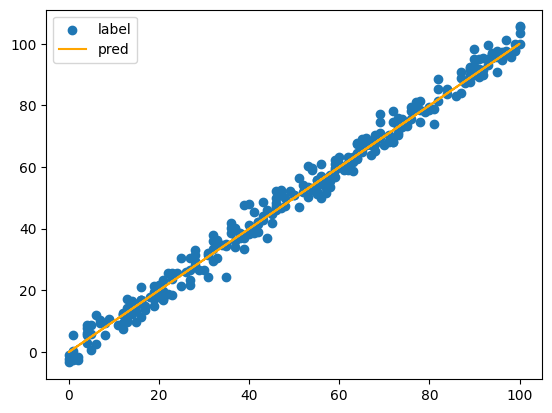
\includegraphics[width=\textwidth]{linear_reg.png}
    \caption{Plot with original data and prediction line}
\end{figure}

\clearpage
\section{Preprocessing the Data}

The data has many features to it.
The first column is the player's name.
The second column is the number of times that player has been at the bat.
The third column is the number of times that player successfully hit a home run.
The fourth column is the number of time that player successfully hit the ball and ran at least one base.
The fifth column is the number of runs batted in. A batter is awarded when his or her plate appearance is a run being scored.
The sixth column is the number of walks completed by a player.
The seventh column is the number of years a player has been playing for.
Other columns include the salary of the player, the player's league and divition.

\section{Models for Hitters}
\subsection{Coefficients of Features}
The coefficients of the linear model are\\
\begin{verbatim}
[-8.98890267e-01,  1.86488487e-01,  1.75640752e-15, -1.80907871e-02,
 -4.45275761e-13, -4.31095009e-02, -5.00041306e-02,  8.73701081e-03,
 6.78644294e-02,  7.91654030e-02,  1.30108646e-01,  1.21687095e-01,
 -1.44953494e-13,  4.68049655e-02,  1.18583569e-01, -2.61721975e-01,
 -1.06220588e-13,  2.92042778e-02, -4.86913597e-02,  9.21115413e-02,
 -4.73956539e-02,  1.27336692e-01,  8.01025912e-14,  1.08095254e-01,
 -1.07239556e-03, -1.42907908e-12,  4.76785278e-13, -9.99591371e-02,
 8.32028890e-13, -4.86497867e-02,  1.40522298e-01,  1.78313597e-02,
 1.94289029e-16, -1.03609685e-01,  1.36700827e-01, -5.80300115e-02,
 1.35626831e-01, -7.76699249e-03, -1.03848861e-01, -8.60088736e-02,
 8.54391219e-02,  3.05311332e-16,  1.24781938e-01, -5.27355937e-16,
 -2.91433544e-16,  1.01915071e-01,  1.02981076e-01, -8.81157809e-03,
 1.15360162e-01, -2.15509913e-02,  8.70187605e-01, -9.14398757e-01,
 -5.22789546e-02, -5.54989486e-02, -4.12631188e-02,  8.25194662e-02,
 3.75133952e-17,  1.33236979e-01, -9.85002214e-03,  1.59184067e-01,
 1.40691263e-01, -4.01685764e-02, -2.00064320e-02, -8.32667268e-17,
 1.59836114e-01,  1.62075128e-01,  8.32667268e-17, -3.58156584e-02,
 -5.28316572e-02,  6.80011603e-16, -3.61802217e-02, -3.34034860e-03,
 5.92456645e-02, -3.41865627e-02, -1.46687749e-02,  2.35922393e-16,
 -4.18326973e-02,  1.12491475e-01, -2.77555756e-16, -5.61049568e-03,
 -5.27702594e-02,  1.39880192e-01,  1.10961336e-02,  1.04530292e-01,
 -5.55372256e-02, -8.87847704e-01, -1.38777878e-16, -3.33066907e-16,
 -1.30538556e-01, -5.29623732e-02, -2.09248356e-02,  6.66783390e-02,
 1.38313065e-01,  5.69807535e-02,  2.18334490e-01, -8.66910892e-01,
 5.55111512e-17, -2.33458278e-02,  3.74700271e-16, -6.87851071e-02,
 -6.79222435e-02,  1.64273129e-01,  1.02935152e-01,  1.48375871e-01,
 1.40672972e-01,  1.55984935e-01, -1.11022302e-16,  9.75751032e-01,
 1.15166545e-01,  9.44457394e-02, -8.15495837e-01, -4.87602223e-02,
 1.94315585e-02,  9.71445147e-17, -1.59594560e-16, -5.88046210e-02,
 -1.34940271e-01,  1.38777878e-17,  9.48134501e-02,  1.11022302e-16,
 -3.99958241e-02,  1.38073738e-01,  9.10243024e-01,  1.03474672e-01,
 -6.13269972e-02,  1.16257972e-01, -5.22903356e-02, -1.01790687e-02,
 4.01004682e-03, -6.31338618e-02, -1.07552856e-16,  5.38745133e-02,
 -7.01510032e-02,  8.59632921e-02, -8.32667268e-17, -3.33066907e-16,
 1.14638940e-01,  6.89214459e-02,  8.94225172e-01, -2.77555756e-16,
 4.29164271e-02, -5.00862186e-02, -5.52247527e-02,  1.06561734e-01,
 1.52655666e-16,  9.81107107e-02, -5.27355937e-16, -4.09726525e-02,
 1.15862393e-01,  9.58194312e-01, -1.06278432e-01, -5.60403280e-02,
 -5.07533331e-02,  3.67761377e-16,  6.57796530e-02,  1.62224083e-01,
 7.52507808e-02, -5.39580504e-02, -9.99353476e-02,  1.12399708e-01,
 -2.97875196e-02, -1.12397888e-01,  1.32068638e-01, -2.83971469e-02,
 -2.62257885e-02,  1.02430735e-01, -1.82768543e-02,  1.12890685e-01,
 5.55111512e-17, -8.58535722e-01, -2.05121635e-02,  7.69287923e-02,
 1.19581936e-01,  1.38777878e-16,  8.32667268e-17,  1.26752565e-01,
 -5.98019787e-02,  6.86595509e-02, -1.11022302e-16,  7.44811401e-02,
 -9.83391610e-02, -6.52298180e-02,  1.97170023e-01,  1.16952568e-01,
 -4.36060871e-02, -3.83485309e-02, -7.84697977e-02, -4.66836509e-02,
 -1.18665770e-01, -9.31138006e-02,  2.16274397e-01,  8.73828710e-02,
 1.06364754e-01,  5.47388116e-02, -3.90594351e-02, -4.16333634e-17,
 -9.19186834e-01, -8.10020707e-03, -5.28652394e-02, -6.06808441e-02,
 0.00000000e+00, -1.11022302e-16, -1.01092365e-02, -2.77555756e-17,
 1.31687721e-01, -3.14649557e-02, -7.08166458e-02, -1.65025700e-02,
 6.93889390e-18, -1.54067330e-01, -7.63165006e-01, -3.10670953e-02,
 -2.96083625e-02,  6.70129290e-02,  9.10352110e-02,  0.00000000e+00,
 0.00000000e+00, -3.14890127e-02, -2.80640605e-03, -1.45766513e-02,
 -3.03401591e-02,  0.00000000e+00,  6.40328919e-02, -5.82525339e-02,
 -5.41572935e-02, -5.75605604e-02, -7.13539658e-02,  0.00000000e+00,
 -1.15476450e-01,  3.93115479e-02,  1.45300069e-01, -8.63534624e-01,
 -7.98957605e-01,  5.67408649e-02,  1.21293473e-01,  8.69728519e-02,
 0.00000000e+00,  1.00516455e-02,  0.00000000e+00,  8.35977449e-02,
 1.06417783e-01,  0.00000000e+00, -2.89477071e-02,  9.71617337e-02,
 -5.62928006e-02,  5.35575714e-02, -2.89387422e-02, -1.04920650e-01,
 2.72861107e-02,  5.25424179e-02, -6.27067191e-02,  9.73210537e-02,
 1.42857291e-02,  1.12308464e-01,  0.00000000e+00,  0.00000000e+00,
 -6.92201151e-02, -7.04690808e-02,  9.61637969e-02,  1.31817497e-02,
 0.00000000e+00, -1.02826861e-01, -1.84472142e-01, -4.27224553e-01,
 4.27224553e-01,  9.39898225e-03, -9.39898225e-03,  4.62088141e-04,
 -1.17275709e-03, -1.08457179e-03, -6.37056483e-05, -7.60176772e-05,
 9.80912524e-04, -3.51738504e-04, -1.33819332e-04,  7.41394903e-04,
 8.44763440e-04, -1.55932803e-04, -3.63137957e-04, -2.21745141e-04,
 1.56603579e-05,  6.15410726e-05, -2.25300948e-03, -4.59214382e-05]
\end{verbatim}

The coefficients of the logarithmic model are\\
\begin{verbatim}
[-7.95737936e-01,  2.18458264e-01,  0.00000000e+00,
-5.34279726e-02,  0.00000000e+00, -5.79006326e-02,
-7.10802682e-02,  5.16715181e-02, -1.51480117e-02,
 7.97663975e-02,  1.12125332e-01,  1.24869216e-01,
 0.00000000e+00,  6.80045721e-02,  1.24768959e-01,
-3.93758384e-01,  0.00000000e+00,  2.63173646e-02,
-5.80898284e-02,  9.97513427e-02, -7.08061992e-02,
 1.54603172e-01,  0.00000000e+00,  1.06665838e-01,
-3.97221186e-02,  0.00000000e+00,  0.00000000e+00,
-9.01968271e-02,  0.00000000e+00, -4.81980938e-02,
 1.45889103e-01,  3.16723557e-02,  0.00000000e+00,
-8.46682781e-02,  1.60317998e-01, -5.20235162e-02,
 1.15587015e-01, -3.61573258e-02, -1.04333430e-01,
-9.25002804e-02,  8.48642549e-02,  0.00000000e+00,
 1.17116882e-01,  0.00000000e+00,  0.00000000e+00,
 9.22131768e-02,  9.49730114e-02, -5.18914925e-02,
 1.39399154e-01, -5.33955233e-02,  7.20974964e-01,
-8.08165901e-01, -6.08432778e-02, -5.23335704e-02,
-4.41447431e-02, -1.30525643e-02,  0.00000000e+00,
 1.57143561e-01, -4.79137047e-02,  1.43295710e-01,
 9.04950917e-02, -5.13917490e-02,  3.44044296e-02,
 0.00000000e+00,  1.36457520e-01,  2.22585565e-01,
 0.00000000e+00, -2.61182417e-02, -4.89388754e-02,
 0.00000000e+00, -5.76994561e-02, -2.98660531e-02,
-2.24912703e-02, -4.43919991e-02, -3.85295036e-02,
 0.00000000e+00, -7.38449501e-02,  1.37825950e-01,
 0.00000000e+00,  2.23129579e-02, -6.36457923e-02,
 1.47893175e-01, -2.75940834e-02,  8.36270112e-02,
-5.30208930e-02, -7.46490347e-01,  0.00000000e+00,
 0.00000000e+00, -1.77659712e-01, -6.59888192e-02,
-5.50143370e-02,  8.77110792e-02,  1.18997304e-01,
 7.79567739e-02,  2.70354224e-01, -7.45777616e-01,
 0.00000000e+00, -5.30108960e-02,  0.00000000e+00,
-7.12919203e-02, -6.76894765e-02,  1.99891851e-01,
 9.39627235e-02,  1.40414904e-01,  1.22164492e-01,
 1.55919963e-01,  0.00000000e+00,  8.47319772e-01,
 1.29589772e-01,  8.17180615e-02, -6.48085047e-01,
-3.82285375e-02, -2.26090753e-02,  0.00000000e+00,
 0.00000000e+00, -5.45433782e-02, -1.22659133e-01,
 0.00000000e+00,  1.02199823e-01,  0.00000000e+00,
-5.67213614e-02,  1.19316261e-01,  8.01828245e-01,
 8.48308242e-02, -5.77530166e-02,  1.11480585e-01,
-4.67642771e-02, -4.48189842e-02,  3.62759138e-02,
-5.60392215e-02,  0.00000000e+00,  5.72975900e-02,
-6.75008080e-02,  1.03025419e-01,  0.00000000e+00,
 0.00000000e+00,  9.15494381e-02,  9.25365000e-02,
 7.65703876e-01,  0.00000000e+00,  4.56905114e-02,
-4.47410173e-02, -6.56853804e-02,  1.32825506e-01,
 0.00000000e+00,  1.02507825e-01,  0.00000000e+00,
-4.23416654e-02,  9.08266371e-02,  8.60410998e-01,
-1.15217245e-01, -5.64275973e-02, -5.47547418e-02,
 0.00000000e+00,  8.27064657e-02,  1.75885412e-01,
 7.79319007e-02, -5.02074815e-02, -9.58156088e-02,
 9.60879464e-02, -5.84771524e-02, -9.15103042e-02,
 1.09158829e-01, -3.76289110e-02, -5.97466321e-02,
 8.01683213e-02, -3.40714719e-02,  1.04059574e-01,
 0.00000000e+00, -7.16132320e-01, -5.68454624e-02,
 7.64390157e-02,  1.15516167e-01,  0.00000000e+00,
 0.00000000e+00,  9.87467879e-02, -5.90177969e-02,
 7.31708593e-02,  0.00000000e+00,  7.45302500e-02,
-7.48497200e-02, -7.40428150e-02,  1.81941073e-01,
 1.19262417e-01, -5.70445301e-02, -4.97469133e-02,
-9.95396441e-02, -5.10476909e-02,  1.35525599e-03,
-8.55729179e-02,  2.30280712e-01,  9.91249704e-02,
 8.29295350e-02,  6.00676881e-02, -4.52508862e-02,
 0.00000000e+00, -8.08117431e-01, -2.89757432e-02,
-6.95572358e-02, -1.01030436e-01,  0.00000000e+00,
 0.00000000e+00, -3.71100389e-02,  0.00000000e+00,
 1.20304887e-01, -4.52342444e-02, -5.55221764e-02,
-4.59378211e-02,  0.00000000e+00, -1.72212691e-01,
-5.47291093e-01, -4.85881710e-02, -4.24773413e-02,
 5.88800759e-02,  9.82556008e-02,  0.00000000e+00,
 0.00000000e+00, -5.26181775e-02,  4.04871236e-02,
-4.96003525e-02, -4.29298265e-02,  0.00000000e+00,
 8.56523654e-02, -6.66705935e-02, -5.49567841e-02,
-6.31308335e-02,  1.42943621e-02,  0.00000000e+00,
-1.12707945e-01,  5.05879319e-02,  9.75509743e-02,
-7.31359712e-01, -7.07510582e-01,  7.10538860e-02,
 7.08405418e-02,  8.88408310e-02,  0.00000000e+00,
-3.55830575e-02,  0.00000000e+00,  8.69656839e-02,
 1.18851899e-01,  0.00000000e+00, -4.32426663e-02,
 9.04514050e-02, -6.10372952e-02,  6.06730219e-02,
-4.19464171e-02, -7.92532574e-02,  5.10432795e-02,
 5.57436598e-02, -6.75667218e-02,  9.78588813e-02,
 5.49890399e-02,  1.27900842e-01,  0.00000000e+00,
 0.00000000e+00, -7.06353240e-02, -7.17027710e-02,
 8.98382796e-02,  4.17249538e-02,  0.00000000e+00,
-8.63873562e-02, -2.19382029e-01, -2.51675490e+00,
 2.33160460e+00, -3.95801861e-02, -1.45570118e-01,
 4.93410850e-03, -1.56850795e-02, -1.76301046e-02,
-2.40899081e-03,  8.27385567e-04,  1.10785528e-02,
-4.94413348e-02, -1.70961434e-03,  1.06098833e-02,
 1.10406725e-02, -3.17898607e-03, -5.77219019e-03,
-1.70442768e-03,  2.72225789e-04,  7.13690072e-04,
-1.90692127e-02, -4.34068327e-04]
\end{verbatim}
The coefficients are different. This is because the linear regression does not fit the data very well. On the otherhand, the logistic regression model fits the data much better.

\subsection{ROC Curves}
\begin{figure}[!ht]
    \centering
    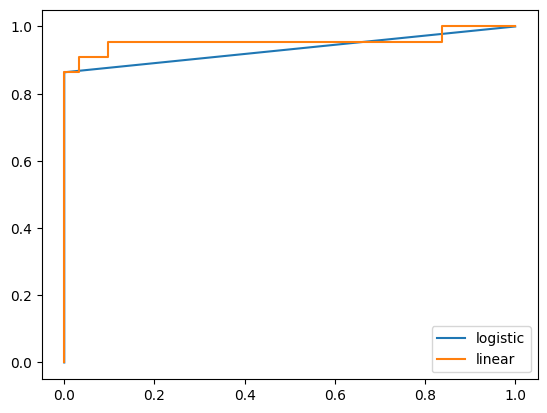
\includegraphics{roc.png}
    \caption{Caption}
\end{figure}

\subsection{Optimal Decision Threshold}
Finding the optimal threshold is finding the largest difference between the true positive rate and the false positive rate. 
The logistic model's optimal threshold is 0.9318181818181819 and the linear model's optimal threshold is 0.9560117302052785

\section*{References}
{
\small
[1] Watt, Jeremy, Borhani, Reza \ \& Katsaggelos, Aggelos Konstantinos\ (2016) Machine Learning Refined.

[2] Konasani, Venkata Reddy \ \& Shailendra Kadre\ (2021) Machine Learning and Deep Learning Using Python and TensorFlow.
}

\end{document}
